\subsection{User Profile Page (Interface Mockup)}

\begin{figure}[h!]
\centering
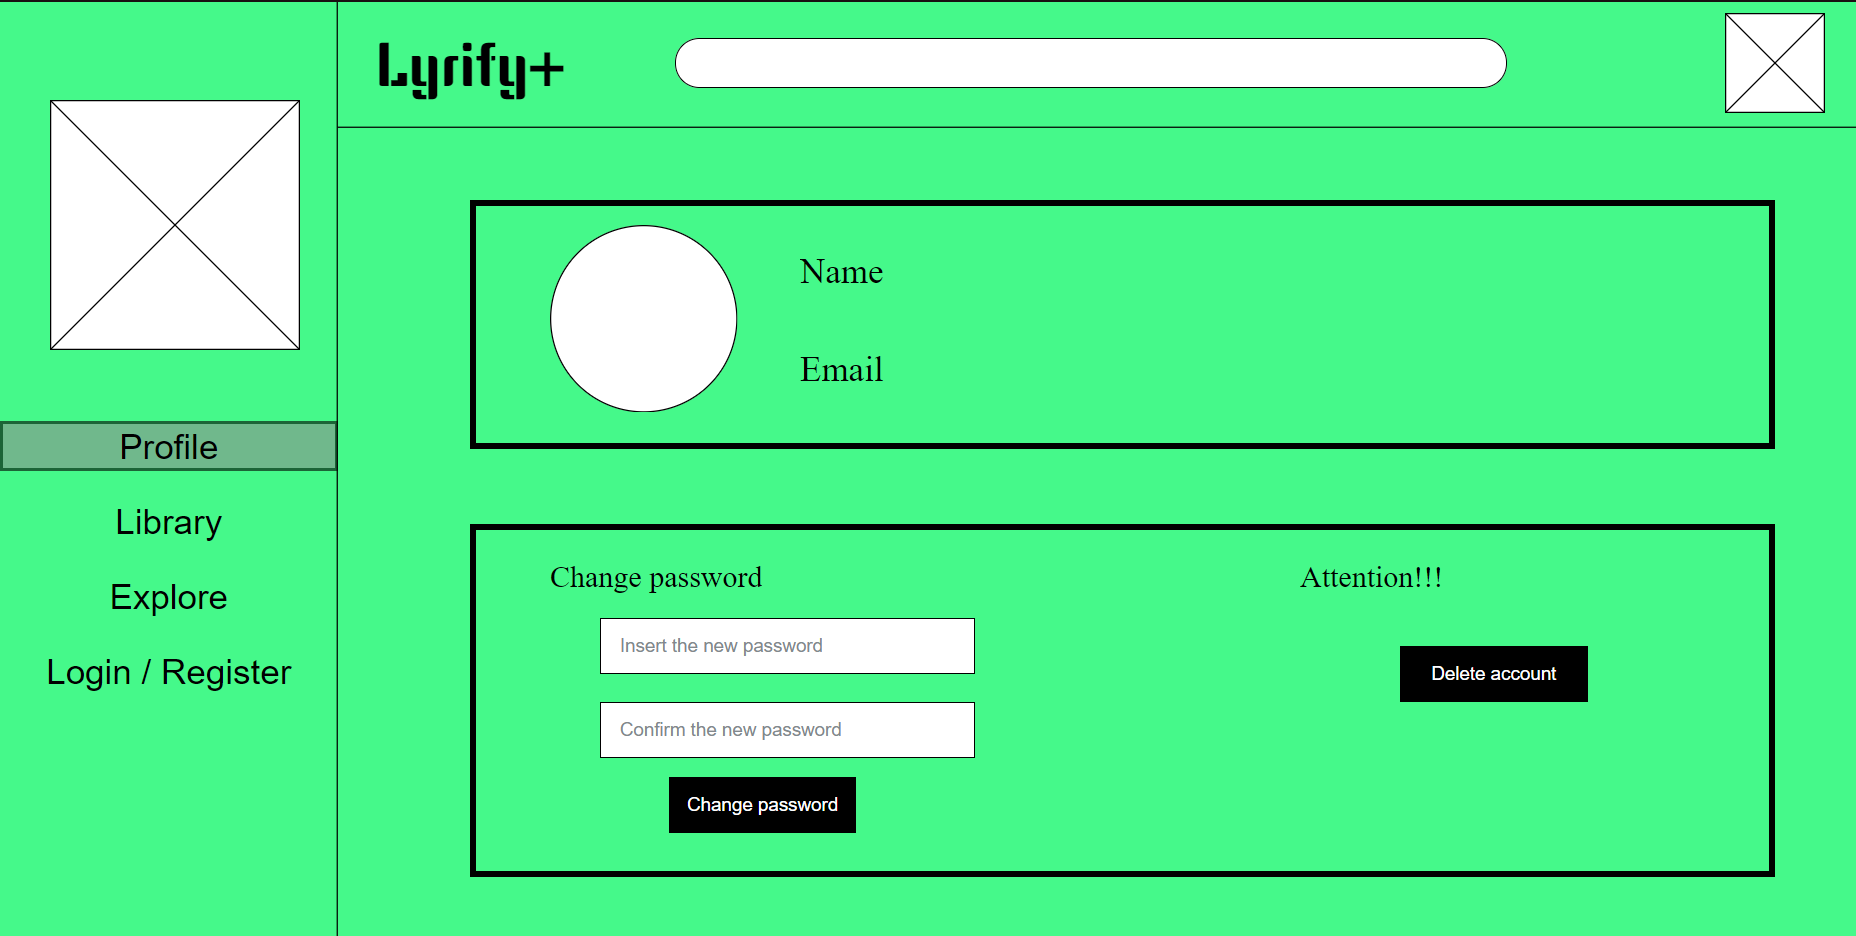
\includegraphics[width=0.9\textwidth]{sections/PLL/ProfilePageMockup.png}
\caption{User profile page}
\end{figure}

On the user's profile page, the menu on the left side will be repeated but with the 'Profile' button darkened to indicate that the user is in that page. Then, the top row is also shown including the app's name, search bar and profile photo. The center of the page will be divided in two parts, the user's information part and the account settings part.
For the user's information part, the profile photo will be displayed in a bigger size along with the username and the mail.
For the account settings part, there will be an option for changing the password by filling both fields and then clicking on the 'Change password' button, that will update our database with the new credentials for the user. In addition, in case the user no longer wants to keep using our app, there will be a 'Delete account' button that will delete all the user's data from our database and will redirect the user to the Login / Register page. 